% !TEX root = pfe-book2.tex
%!TEX TS-program = pdflatex
%!TEX encoding = UTF-8 Unicode


\cleardoublepage
%\mainmatter
\chapter{Giant Molecules}
\label{ch-09}

\section{Chains of Atoms}

Chemists and technologists have been dealing for a long time with natural substances consisting of long molecules in which the atoms are bound like the links of a chain. We find examples on every hand: abundant substances as rubber, cellulose and protein constitute chain-type molecules made up of many thousands of atoms. The structural conceptions of such molecules were formed and developed in the twenties, when chemists learned to produce such substances in their laborato­ries.

One of the first steps in producing substances built of long-chain molecules was the creation of synthetic caout­chouc. This brilliant research was completed in 1926 by the Soviet chemist Sergei Vasilyevich Lebedev (1874-1934). The industrial production of synthetic caoutchouc (as crude rubber is called) was a vital problem in the USSR as it was in great demand for the manufacture of automobile tires (rubber is made of caoutchouc, or crude rubber) and because the rubber tree requires a tropical climate for its cultivation.

The hevea, or simply rubber, tree flourishes in the Brazilian jungle and from it oozes latex, a milky liquid that is a suspension of crude rubber. The Brazilian Indians made balls of crude rubber and also used it for making footwear. But in 1839, Charles Goodyear (1800-1860) originated the process for vulcanizing crude rubber. Treating crude rubber with sulphur and subjecting it to heat convert the sticky plastic crude rubber into elastic rubber.

At first the demand for rubber was low, but today mankind requires millions of tons annually. As we have already mentioned, rubber trees grow only in tropical forests so that countries in cold or temperate zones must produce synthetic rubber in plants on an industrial scale to avoid dependence on crude rubber imports.

To produce synthetic crude rubber, it is necessary, of course, to know what crude rubber (caoutchouc) is. When Lebedev began his investigations, the chemical formula of crude rubber was already known. It has the following form:

%\setatomsep{2.5em}
\hspace{-20pt}{\scriptsize
\chemfig{-[:60]CH_{2}-CH_{2}-[:-60]C(-[:-120]CH_{3})=CH-[:60]CH_{2}-CH_{2}-[:-60]C(-[:-120]CH_{3})=CH-[:60]CH_{2}-CH_{2}-[:-60]C(-[:-120]CH_{3})=CH-[:60]} \par}

The chain shown here has neither beginning nor end. We see that the molecules are built up of identical links. We can therefore write the formula for crude rubber in a more concise form:
\begin{center}
{\scriptsize
\chemleft[\chemfig{-CH_{2}-C(-[:270]CH_{3})=CH-CH_{2}@{c2}-}\chemright]\chemmove{
    \node at ([shift={(30pt,-24pt)}]c2.south east) {$n$};
}\par}
\end{center}

%{\tikz{\draw[line width=1.5pt, ,<->, orange] (0, 0) --
%    (.75,0);}}
The quantity $n$ may reach many thousands. Long-chain molecules built of repeating groups are called \emph{polymers}. 

An enormous number of synthetic polymers have found most extensive application in engineering and in the textile industries. They include nylon, polyethylene, capron, polypropylene, polyvinyl chloride and many, many others.

Of simplest structure are the molecules of polyethylene. Bags of this material are found in the kitchen tables of houses and apartments almost all over the world. If a molecule of polyethylene is stretched as far as it will go, it resembles the illustration in \figr{fig-9.1}. As you can see, physicists were able to determine the distances between the atoms and the angles between the valence bonds.

\begin{figure}[!ht]
\centering
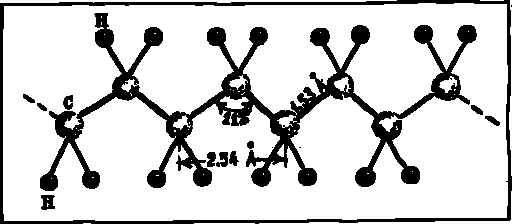
\includegraphics[width=\textwidth]{figures/fig-09-01.pdf}
\caption{A molecule of polyethylene.}
\label{fig-9.1}
\end{figure}

Long-chain molecules are not necessarily polymers, i.e. they do not necessarily consist of repeating groups. Chemists have learned to ``design'' molecules built up of two or more different groups. If the groups alternate in a definite order, for example, according to the ar­rangement $ABABABABAB$, it is still appropriate to call such a molecule a polymer. We often deal, however, with molecules not having such an ordered sequence. Can we call a molecule with the arrangement $ABBBABABAAABBBBABABAABBA$ a polymer? This, however, is a matter of taste and tastes in names may differ.

A natural protein molecule is rarely called a polymer. Proteins are built up of some twenty pieces of different kinds. These pieces, or building blocks, are called amino acid radicals.

There is one essential difference between protein mole­cules and synthetic molecules built up of several pieces arranged in disorder. No two molecules are the same in a piece of synthetic polymer. Such a chain molecule may consist of one random sequence of component pieces, with another, different random sequence in another mol­ecule, This usually has a detrimental effect on the prop­erties of the polymer. If the molecules do not resemble one another, they cannot be efficiently packed together. In principle, such molecules cannot build up a crystal. Substances of this type produce amorphous glasses.

In the last decades, chemists have learned to build regular polymers, and have thus made many valuable materials available to industry.

As to natural proteins of a definite type (say the hem­oglobin of a bull), the molecules are all the same even though they have a disordered structure. A molecule of protein of a given sort can be compared to a page of a book: the letters follow one another in a random, but quite definite order. All the molecules of a protein are copies of the same page of the book.

\section{Flexibility of Molecules}

A long-chain molecule can be likened to a rail. A line \SI{0.1}{\milli\meter} long can accommodate a million atoms. The crosswise dimension of a molecule of polyethylene is about 3 or \SI{4}{\angstrom}. Thus the length of the molecule is greater than its width by several hundred thousand times. Since a rail of the kind used in railways has a thickness of about \SI{10}{\centi\meter}, with the same length-to-thickness ratio as the molecule, the rail would have to be \SI{10}{\kilo\meter} long.

This does not imply, of course, that there are no short­er polymer molecules. Unless special measures are taken, we find in a polymer substance molecules of different lengths, from one consisting of several groups to those built up of thousands of groups.

\begin{figure}[!ht]
\centering
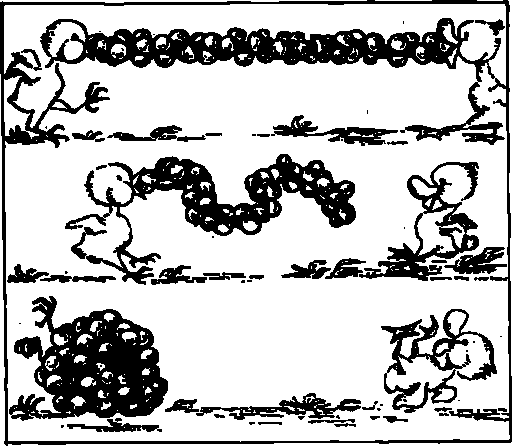
\includegraphics[width=\textwidth]{figures/fig-09-02.pdf}
\caption{A flexible polymer molecule.}
\label{fig-9.2}
\end{figure}
We likened a long-chain molecule to a rail. In another sense, this is not a very apt comparison. A rail is diffi­cult to bend, while a molecule bends easily. The flexibil­ity of a macromolecule is not similar to that of a willow switch. The molecule owes its flexibility to a capacity possessed by all molecules: one part of the molecule can swivel about another part if they are joined by bonds that chemists call single (monovalent) bonds. We can readily understand that this property of polymer mol­ecules enables them to assume the queerest shapes. Illustrated in \figr{fig-9.2} is a model of a flexible molecule in three positions. If a molecule is suspended in a solution, it is usually coiled into a ball.

The stretching of a rubber band consists in the uncoiling of its molecules. Thus, the flexibility of polymers is of an entirely different nature than that of metals. If the stretched band is released, it contracts to its former length. Hence, the molecule tends to go over from its linear (stretched) shape to a coiled one. Why does this occur? There are two possible reasons. In the first place, we can assume that the coiled shape is more advantageous from energy considerations. In the second place, we can sup­pose that coiling contributes to an increase in entropy. Hence, which law of thermodynamics governs this be­haviour: the first or the second? Evidently, both. But the coiled state is doubtlessly advantageous from the entropy viewpoint as well. Obviously, the sequence of the atoms of molecules coiled into a ball is in more disorder than when the molecules are stretched out in a straight line. We also know that disorder and entropy are closely re­lated.

\section{Globular Crystals}

Many molecules are capable of winding up into tight coils or, as they are sometimes called, globules. Very neat and quite identical globules make up a protein molecule. There is one subtle reason for this. As a matter of fact, a protein molecule contains parts that ``like'' water, and other parts that have an aversion to water. The parts that do not ``like'' water are said to be hydrophobic. The coiling of the protein molecules is governed by a single tendency: all the hydrophobic parts are to be hidden in­ side the globule. This is why the globules in a solution of protein resemble one another like identical twins.


\begin{figure}[!ht]
\centering
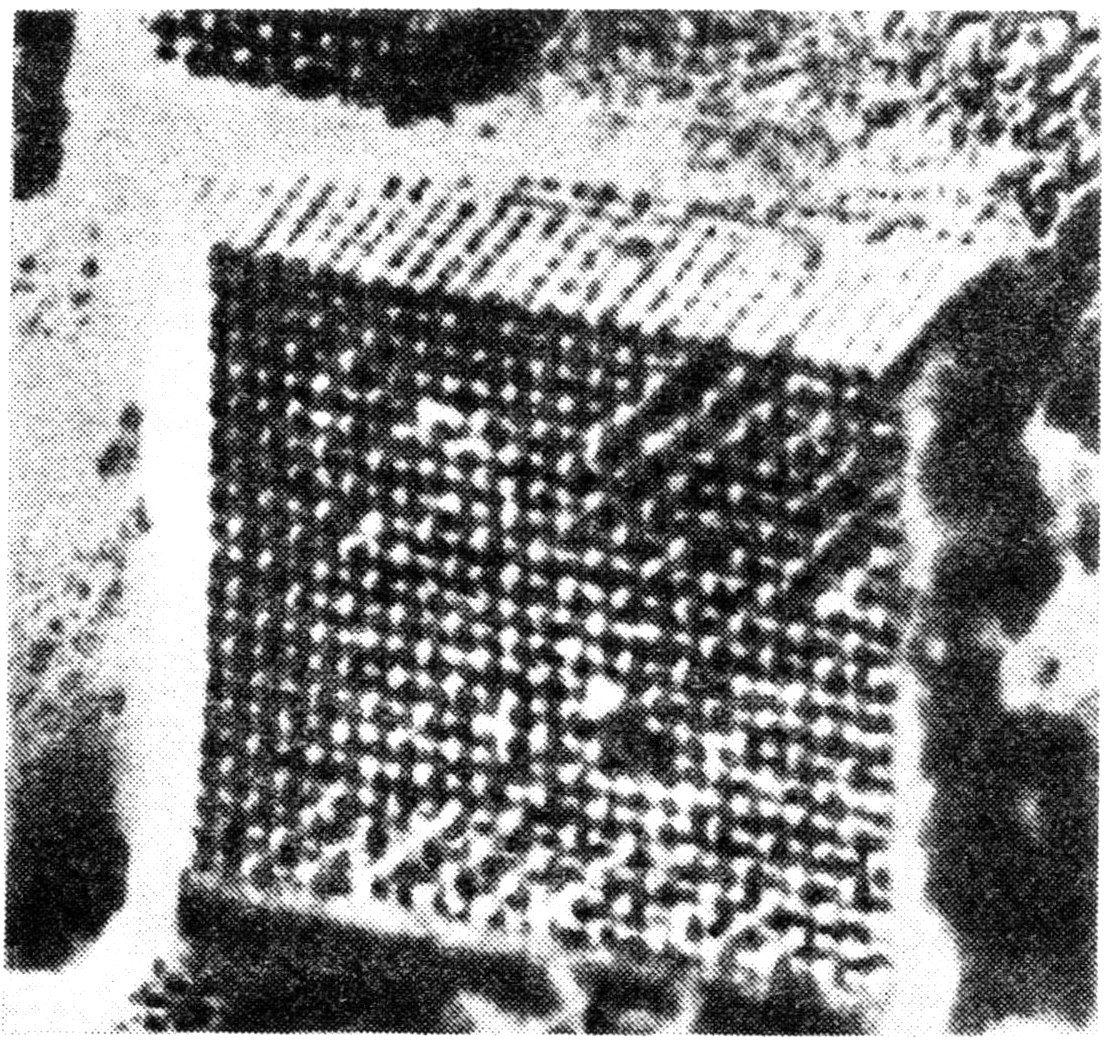
\includegraphics[width=0.4\textwidth]{figures/fig-09-03.jpg}
\caption{An electron micrograph of a tobacco mosaic virus.}
\label{fig-9.3}
\end{figure}

Protein globules are more or less spherical. The size of a globule ranges from 100 to \SI{300}{\angstrom}, making it readily visible under an electron microscope. The first elec­tron micrographs of globular crystals were obtained several decades ago, when electron microscopy tech­niques were considerably less advanced than they are to day. Such a photograph of the tobacco mosaic virus is shown in \figr{fig-9.3}. A virus is more complex than a protein, but this example is quite suitable to illustrate our point, the tendency of biological globules to an ex­ceptionally high degree of order.


But why haven’t the authors provided a micrograph of a protein crystal? The answer is simple. Protein crys­tals are absolutely extraordinary. They contain an im­mense amount of water (sometimes up to 90\%). This makes it impossible to photograph them in an electron microscope. Protein crystals can be investigated only by manipulating them in a solution. A tiny flask contains the solution and a monocrystal of the protein. This object can then be studied by all available physical methods, including $X$-ray structure analysis, which we have re­peatedly mentioned.

Notwithstanding the huge amount of water -- ordinary water, no different from tap water -- the globular protein molecules are arranged in absolutely strict order. Their orientation to the axis of the crystal is the same for all the molecules. We have already mentioned that the mol­ecules are identical. This superior order enables the structure of the protein molecule to be determined. This is no simple task and the investigators Max Ferdinand Perutz (1914-2002) and John Cowdery Kendrew (1917-1997), the first to determine the detailed structure of haemoglobin and myoglobin, were awarded a Nobel prize for their work.

The structure of about a hundred protein molecules is known today. Research continues in this field. Alto­gether, there are about ten thousand different proteins in a living organism. The activity of the living organism depends upon the way in which the proteins are coiled and in which order the different amino acid radicals follow one another in the molecule. No doubt that research con­cerning the structure of protein molecules will continue until all the details of the ten thousand kinds of molecules that govern life processes have been completely cleared up.

\section{Bundles of Molecules}

If molecules can be closely packed when they are stretched to the limit, the solid polymer material they comprise can form various quite complex structures that pos­sess one common property. The solid body contains more or fewer regions in which the molecules adjoin one ano­ther like a bundle of pencils held in the fist.

Depending upon the percentage of such bundle-type regions in the body, and on how neatly the molecules com­prising each such region are packed, the polymer pos­sesses a certain ``degree of crystallinity''. Most polymers object to being simply classified as either amorphous or crystalline solids. There is nothing strange in this because we are dealing with giant molecules and, moreover, mostly of different kinds. Ordered (``crystalline'') regions in polymers can be roughly divided into three classes: bundles, spherulites and crystals of folding molecules.

\begin{figure}[!ht]
\centering
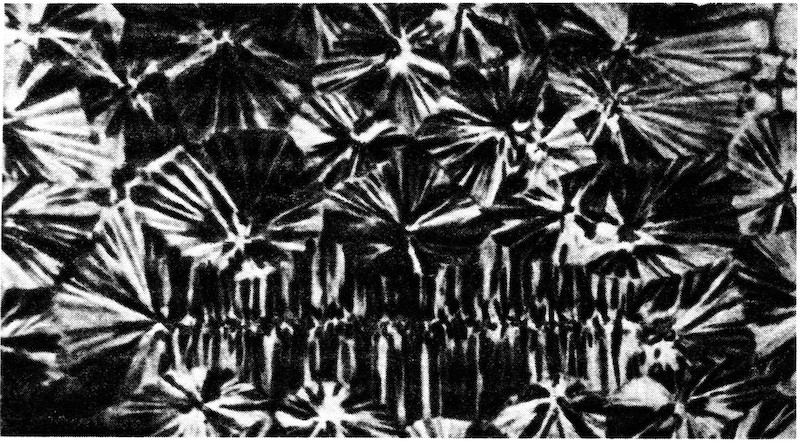
\includegraphics[width=\textwidth]{figures/fig-09-04.jpg}
\caption{A typical microstructure of a polymer.}
\label{fig-9.4}
\end{figure}

A typical microstructure of a polymer is shown in \figr{fig-9.4}. This photograph has been magnified 400 times and was made from a film of polypropylene. The star-shaped figures are kinds of crystallites. The growth of the spherulite began from the centre of the star as the polymer was cooled. Then the spherulites met and interfered with one another’s growth. Consequently, they did not acquire a perfect spherical shape (if you succeed in observing the growth of a separate spherulite, you will actually see a sphere, so that the name is justified). Inside the spheru­lite, the long molecules are arranged with sufficient neat­ ness. Most likely, a spherulite can be envisioned as a neatly coiled rope. The rope represents a bundle of mol­ecules. Thus the long axis of the molecules is positioned perpendicular to a radius of the spherulite. On the same  photograph we see lamellar regions. These may consist of bundles of molecules, or they may be crystals of fold­ ing molecules. The existence of such crystals is, per­ haps, one of the most interesting and absolutely authen­tic facts concerning the structure of polymers.

The following outstanding discovery was made twenty years ago. Small crystals of various polymer substances were separated out of solutions. The investigators were astonished to find that the same kind of crystals, with a surface resembling a winding staircase, grew from solu­tions of various paraffins. What is the cause of spiral growth of crystals which look like they had been prepar­ed by a skilled pastry-cook (\figr{fig-9.5})?

\begin{figure}[!ht]
\centering
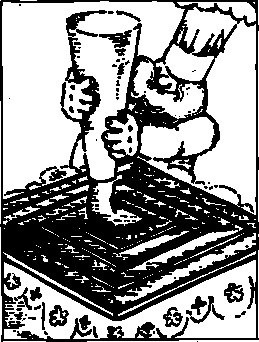
\includegraphics[width=0.4\textwidth]{figures/fig-09-05.pdf}
\caption{A spiral growth in polymer crystals.}
\label{fig-9.5}
\end{figure}

When we discussed crystal growth on page~\pageref{fig-4.6}, we omitted one important circumstance. Imagine that a growing plane (face) of a crystal is completely filled with atoms. No positions remain that attract new atoms strongly enough. This being the case, it can be calculated that growth should proceed at an inconceivably slower rate than that actually observed. This contradiction between theory and practice was finally solved: such rapid crystal growth was found possible when there are screw disloca­tions in the growing crystal. If there is a screw disloca­tion, the faces grow so that the steps at which new atoms can be readily attached never grow out to the edge of the crystal where they disappear. Physicists were certainly relieved when screw dislocations extricated them from their dilemma. The growth rates became clear as did the essence of the winding staircase feature indicated above for pa­raffin. Such spiral pyramids are frequently observed, and there is nothing strange about the fact that they exist.

Nothing strange while we are referring to crystals built up of small molecules. The explanation is appropri­ate for such crystals: the size of the molecules, height of the steps and the thickness of the crystal are all data that do not contradict one another.

But, when such a picture of crystal growth is observed in a polymer, it is, at first, puzzling. The point is that the thickness of the layers of polyester ranges from 100 to \SI{120}{\angstrom}, while the length of the molecule is \SI{6000}{\angstrom}. What conclusion can we reach on the basis of these fig­ures? There is only one feasible explanation: the molecules are folded in these crystals. The flexibility of the mole­cules enables them to fold without difficulty. All that re­mains is to ponder (and such pondering continues to the present day) over the choice of the most suitable of the three models illustrated in \figr{fig-9.6}. The differences between the models are only minor ones. However, a spe­cialist in this field will resent such a statement. ``How can you call them minor?'' he will object. ``In the upper drawing, the molecules are folded over haphazardly, skip­ ping their nearest neighbours; in the second model, the molecules become their own neighbours. The difference between the second and third models is that the surface of the crystal is smoother in the middle drawing than in the lower one.''

\begin{figure}[!ht]
\centering
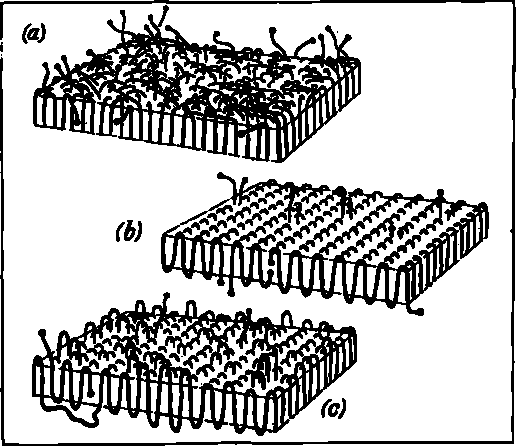
\includegraphics[width=0.9\textwidth]{figures/fig-09-06.pdf}
\caption{Models for folding of polymer molecules in crystals.}
\label{fig-9.6}
\end{figure}

The specialist is right: the packing or stacking arrange­ment of polymer molecules is of exceptional significance and has a fundamental effect on the properties of the sub­ stance. Although polyethylene, nylon and like materials were first synthesized several decades ago, the study of their supramolecular structure and investigation in the techniques required to pack the molecules in different ways are being continued to this day by many scientists in this field.

\section{Muscular Contraction}

We shall complete our discussion on giant molecules by considering an example that demonstrates how macro­ molecules behave in a living organism.

Biologists considered it to be their task to explain the conformity of the shapes of living organs -- for instance, the shape of the hand or a leaf of a tree -- to the functions of the organs.

Physicists, having decided to apply methods for in­vestigating the structure of matter and the laws of nature in studying processes that occur in living organisms, are making efforts to understand life at the molecular level. The structure of tissues can be investigated today in great detail. After establishing the structure, it becomes feasible to develop a model of biological events.
\begin{figure}[!ht]
\centering
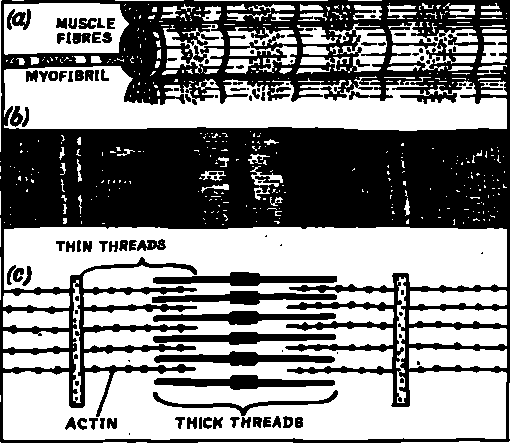
\includegraphics[width=\textwidth]{figures/fig-09-07.pdf}
\caption{How muscles contract?}
\label{fig-9.7}
\end{figure}

A quite significant achievement in this line is the advance­ment of the theory of muscular contraction. The mus­cle fibre consists of two types of threads: thin ones and thick ones (\figr{fig-9.7}~\hlgray{(a)}). The thick threads consist of pro­tein molecules called myosin. Physicists have estab­lished that a myosin molecule has the shape of a rod with a thickening at the end. In the thick thread, the mole­cules join with their thickened tails in the middle (\figr{fig-9.7}~\hlgray{(c)}). The thin threads consist of actin whose structure resembles two strings of beads forming a double helix. Muscle contraction consists in the thick threads sliding into the helixes of the thin threads.


The details of this mechanism are known, but we cannot discuss them here. The signal for a muscle contraction is given by a nerve pulse. Its arrival releases atoms of cal­cium which transfer from one part of the thread to another. As a result, the molecules turn towards one another so that it becomes advantageous from an energy viewpoint for one set of molecules to slide into the other set. The illustration gives two schematic diagrams with an elec­tron photomicrograph (\figr{fig-9.7}~\hlgray{(b)}) between them.

I fear that these pages provide only a faint idea of the degree of detail to which the mechanism of muscle con­traction has been studied. But our aim was only to in­terest the reader. Consider the last page of this book de­voted to molecules as only a preview of a detailed discus­sion on biological physics which we hope to include in one of the subsequent books of \emph{Physics for Everyone}.